\documentclass[tikz,14pt,border=10pt]{standalone}

\usepackage{verbatim}
\usepackage{textcomp}
\usetikzlibrary{arrows,positioning}

\begin{document}

\tikzset{
  coords/.style = {coordinate},
  block/.style    = {draw, thin, rectangle, minimum height = 6.4em,
    minimum width = 7em},
  frame/.style   = {coordinate},
  arrow/.style={thick, ->, >=stealth'}
}

\begin{tikzpicture}
  \node[anchor=south west,inner sep=0, name=image] at (0,0) {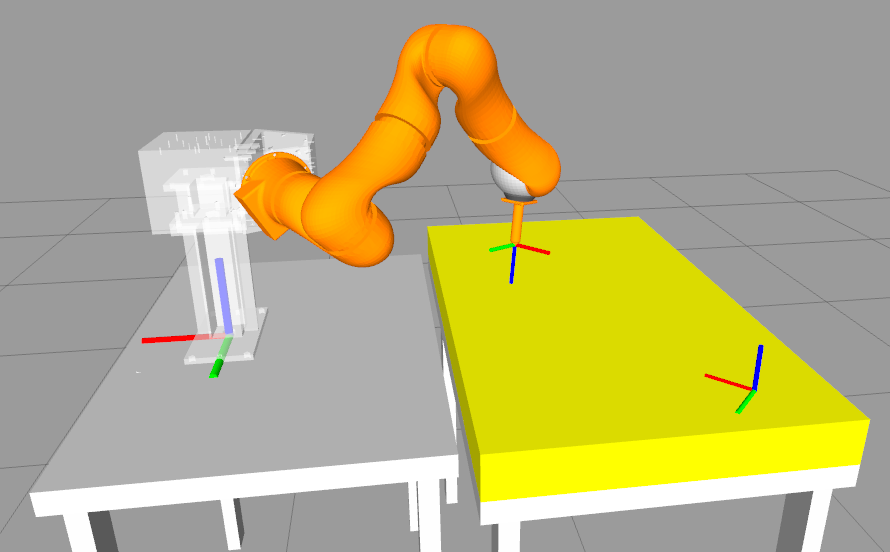
\includegraphics[width=\textwidth]{whole_robot.png}};
  \node[coords, name=origin]{};
  \node[above right = 4.9cm and 9cm of origin] {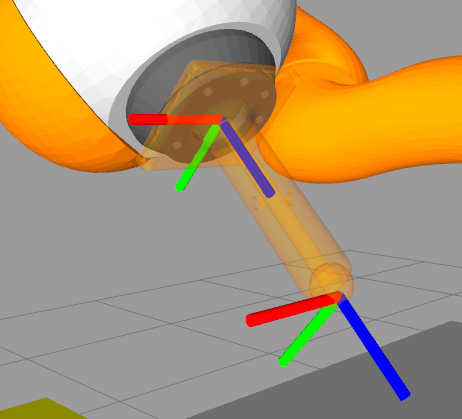
\includegraphics[scale=0.15]{ee_zoom.png}};
  \node[block, above right = 5cm and 9.1cm of origin] (bounding_box){};
  \node[frame, above right = 2.97cm and 3.13cm of origin](vito_anchor){};
  \node[frame, above right = 4.19cm and 7.04cm of origin](ee){};
  \node[frame, above right = 2.22 and 10.29cm of origin](ws){};

  \node[below left = -1.9cm and -2.35cm of bounding_box, color=black](ws_text){$\{S_{fl}\}$};
  \begin{scope}[transparency group, opacity=0.8]
    \node[above right = 2.37cm and 2.1cm of origin](vito_anchor_text){$\{S_{b}\}$};
    \node[above right = 4.1cm and 7.04cm of origin](ee_text){$\{S_{ee}\}$};
    \node[above right = 2.0cm and 10.29cm of origin](ws_text){$\{S_{ws}\}$};
    \draw[arrow](vito_anchor) -- node [pos=0.5, below = 0cm of ee]{\Large $p_{ee}$}(ee);
    \draw[arrow](vito_anchor) -- node [pos=0.5, below = -0.05cm of ws]{\Large $p_{ws}$}(ws);
    \draw[arrow](ws) -- node [pos=0.55, below = 0cm of ee]{\Large $r$}(ee);
  \end{scope}
\end{tikzpicture}

\end{document}
